\documentclass[crop]{standalone}

\usepackage[dvipsnames]{xcolor}
\usepackage{tikz}

\usetikzlibrary{backgrounds}

\begin{document}
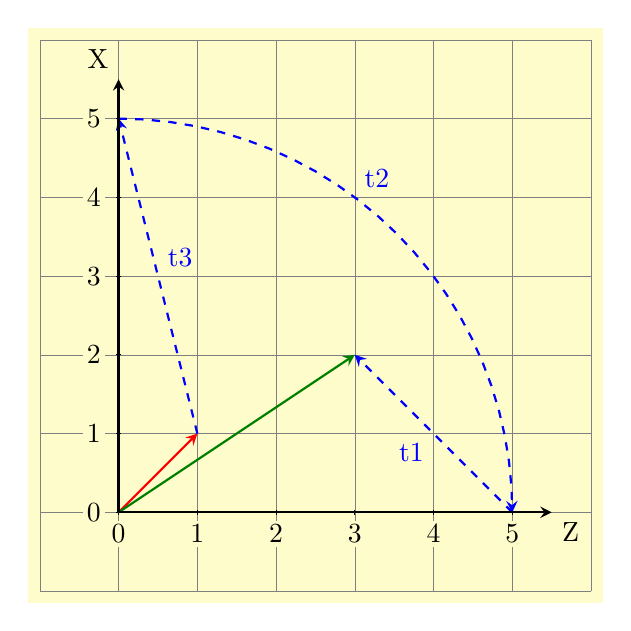
\begin{tikzpicture}[background rectangle/.style={fill=yellow!20}, show background rectangle]


	\draw[step=1cm,gray,very thin] (-1,-1) grid (6,6);

	\foreach \z in {0,1,2,3,4,5}
		\draw (\z cm,1pt) -- (\z cm,-1pt) node[anchor=north, inner sep=1.5pt, outer ysep=2pt, fill=yellow!20] {$\z$};
	\foreach \x in {0,1,2,3,4,5}
		\draw (1pt,\x cm) -- (-1pt,\x cm) node[anchor=east, inner sep=1.5pt, outer xsep=4pt, fill=yellow!20] {$\x$};

	\draw[thick,-stealth,red] (0,0) -- (1,1);
	\draw[thick,-stealth,blue,dashed] (1,1) -- (0,5);
	\draw[blue,thick,domain=90:0,dashed,-stealth] plot ({5*cos(\x)}, {5*sin(\x)});
	\draw[thick,-stealth,blue,dashed] (5,0) -- (3,2);
	\draw[thick,-stealth,Green] (0,0) -- (3,2);
	\node[blue,anchor=south west] at (0.5,3) {t3};
	\node[blue,anchor=south west] at (3,4) {t2};
	\node[blue,anchor=north east] at (4,1) {t1};

	\draw[thick,-stealth] (0,0) -- (5.5,0) node[anchor=north west] {Z};
	\draw[thick,-stealth] (0,0) -- (0,5.5) node[anchor=south east] {X};


\end{tikzpicture}
\end{document}
